\newpage
\section{Metodolog\'ia}

\subsection{Descripci\'on de los datos}

\subsubsection{Lectura y estandarizaci\'on de los datos}
El an\'alisis se hizo en base a un dataset de licencia abierta obtenido de los datos abiertos del gobierno.
Contiene las siguientes especificaciones:



\begin{tabular}{|l|l}
\rowcolor[HTML]{C0C0C0} 
\textbf{Campo}                        & \textbf{Valor}                       \\ \hline
\'Ultima actualizaci\'on                  & hace 6 horas                         \\ \hline
Formato                               & CSV                                  \\ \hline
Licencia                              & Libre Uso                            \\ \hline
Estado                                & Activo                               \\ \hline
Fecha de \'ultima modificaci\'on de datos & 2019-08-23T00:00:00Z                 \\ \hline
Periodo de actualizaci\'on              & R/P3M                                \\ \hline
Periodo cubierto por los datos        & De 2005-03-01 a 2019-06-30           \\ \hline
Id                                    & c2d04700-b335-4f95-8e23-baf4e04cd6b7 \\ \hline
Id del Paquete                        & 96e6a1e1-0de2-4656-9fba-f93b9a176f85 \\ \hline
Id de Revisi\'on                        & 21b0794e-99f4-49a6-a6f7-bf14b3a24de0 \\ \hline
\end{tabular}
\caption{}
\label{tab:my-table}
\\
\\
La serie estad\'istica presenta la poblaci\'on que tiene una actividad economica subordinada y remunerada del pais para cada una de las entidades federativas, desglosada por sexo, grupos de edad y cual es el nivel de ingreso de la poblaci\'on.\ref{fig:TrainingDataSet}\cite{datosAbiertos_2019}
\\
\begin{figure}[h!]
	\centering
	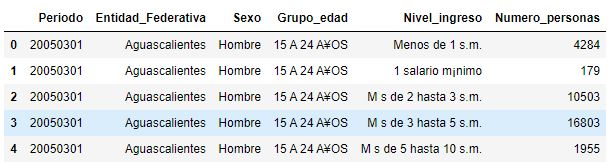
\includegraphics[width=1\linewidth]{Figure/InitialDataSet_Standarization.JPG}
	\caption{Fragmento del dataset utilizado sin procesar.}
	\label{fig:InitialDataSet}
\end{figure}

Con el objetivo de poder utilizar la informaci\'on fue necesario generar una estandarizaci\'on para las columnas, estados, espacio temporal. 
Las columnas se estandarizaron de la siguiente manera:


\begin{lstlisting}[language=Python]
data = pd.read_csv(data_path, encoding='latin1').rename(
    columns = {
        "Periodo": "t",
        "Entidad_Federativa": "state",
        "Sexo": "gender",
        "Grupo_edad": "age",
        "Nivel_ingreso": "wage_level",
        "Numero_personas": "population"
    }
)
\end{lstlisting}

Se detectaron las diferencias este los estados y unific\'o con el siguiente c\'odigo:

\begin{lstlisting}[language=Python]
# Standardize state variable
standardize_state = {
    'Coahuila': 'Coahuila de Zaragoza',
    'Ciudad de M\x82xico': 'Distrito Federal',
    'Estado de M\x82xico': 'M\'exico', 
    'Michoac\xa0n': 'Michoac\'an de Ocampo', 
    'Nuevo Le¢n': 'Nuevo Le\'on',
    'Queretaro': 'Quer\'etaro', 
    'San Luis Potos¡': 'San Luis Potos\'i', 
    'Veracruz': 'Veracruz de Ignacio de la Llave',
    'Yucat\xa0n': 'Yucat\'an'
}

data['state'] = [standardize_state.get(s, s) for s in data.state]
\end{lstlisting}

Se sigui\'o el mismo proceso con el resto de las variables dentro del dataset:
\begin{lstlisting}[language=Python]
# Standardize year variable
data['year'] = [int(str(y)[:4]) for y in data.t]

# Standardize age variable
standardize_age_dictionary = {age_val: age_val.replace("A¥OS", "").replace(" ", "") for age_val in data.age.unique()} 
data['age'] = [standardize_age_dictionary[age] for age in data.age]
\end{lstlisting}

De igual forma se limpiaron los datos de informcai\'on poco relevante para el estudio ('Nacional', No especificado, y NO ESPECIFICADO).

Campo estado ( ver figura \ref{fig:stateUnique_Standarization})

\begin{figure}[h!]
	\centering
	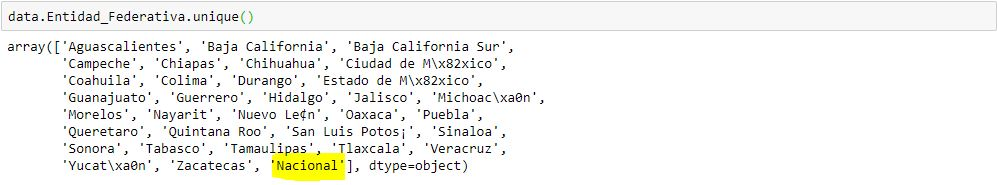
\includegraphics[width=1\linewidth]{Figure/stateUnique_Standarization.JPG}
	\caption{Valores que se limpiaron del dataset a trav\'es de la eliminaci\on de sus respectivas las filas}
	\label{fig:stateUnique_Standarization}
\end{figure}

Campo Salario ( ver figura \ref{fig:wageUnique_Standarization})
\begin{figure}[h!]
	\centering
	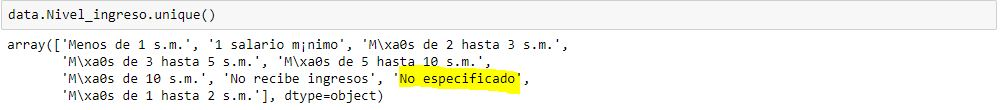
\includegraphics[width=1\linewidth]{Figure/wageUnique_Standarization.JPG}
	\caption{Valores que se limpiaron del dataset a trav\'es de la eliminaci\on de sus respectivas las filas}
	\label{fig:wageUnique_Standarization}
\end{figure}

Campo edad ( ver figura \ref{fig:ageUnique_Standarization})
\begin{figure}[h!]
	\centering
	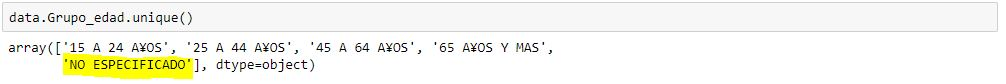
\includegraphics[width=1\linewidth]{Figure/ageUnique_Standarization.JPG}
	\caption{Valores que se limpiaron del dataset a trav\'es de la eliminaci\'on de sus respectivas las filas}
	\label{fig:ageUnique_Standarization}
\end{figure}

\subsubsection{Visualizaci\'on de los datos estandarizados}
Despues de estandarizar los datos 
\begin{figure}[h!]
	\centering
	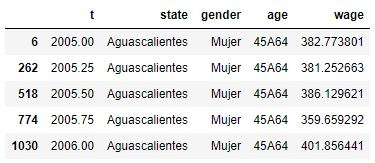
\includegraphics[width=0.8\linewidth]{Figure/AGSdatos_visualizacion.JPG}
	\caption{Datos usados para las graficas de las figuras} \ref{fig:AGSwageVSyear}, \ref{fig:AGSIncrementsVSyear} 
	\label{fig:AGSdatos}
\end{figure}

\begin{figure}[h!]
	\centering
	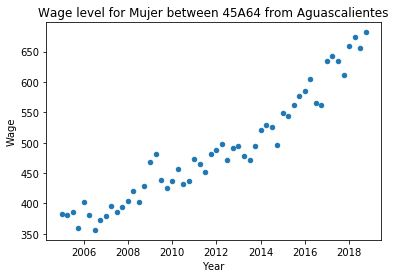
\includegraphics[width=0.8\linewidth]{Figure/AGSwageVSyear_visualizacionJPG.JPG}
	\caption{Salario en funcion del año usando un subconjunto de datos aleatorio} 
	\label{fig:AGSwageVSyear}
\end{figure}

\begin{figure}[h!]
	\centering
	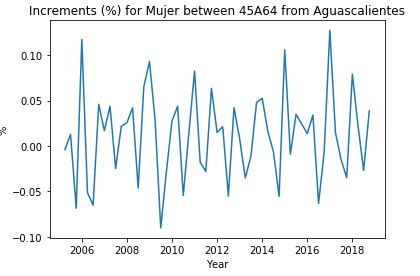
\includegraphics[width=0.8\linewidth]{Figure/AGSIncrementsVSyear_visualizacion.JPG}
	\caption{Incremento en funcion del año usando un subconjunto de datos aleatorio} 
	\label{fig:AGSIncrementsVSyear}
\end{figure}


\subsubsection{Autocorrelaci\'on Parcial}
Las gr\'aficas de autocorrelaci\'on y autocorrelaci\'on parcial se usan mucho en el an\'alisis y pron\'ostico de series de tiempo.
Estas son gr\'aficas que resumen gr\'aficamente la fuerza de una relaci\'on con una observaci\'on en una serie de tiempo con observaciones en pasos de tiempo anteriores. La diferencia entre la autocorrelaci\'on y la autocorrelaci\'on parcial puede ser dif\'icil y confusa para los principiantes con el pron\'ostico de series de tiempo.

Una autocorrelaci\'on parcial es un resumen de la relaci\'on entre una observaci\'on en una serie de tiempo con observaciones en pasos de tiempo anteriores con las relaciones de observaciones intermedias eliminadas.

La autocorrelaci\'on parcial en el retraso k es la correlaci\'on que resulta despu\'es de eliminar el efecto de cualquier correlaci\'on debido a los t\'erminos en los retrasos m\'as cortos.

La autocorrelaci\'on para una observaci\'on y una observaci\'on en un paso de tiempo anterior comprende tanto la correlaci\'on directa como las correlaciones indirectas. Estas correlaciones indirectas son una funci\'on lineal de la correlaci\'on de la observaci\'on, con observaciones en pasos temporales intermedios.

Son estas correlaciones indirectas las que la funci\'on de autocorrelaci\'on parcial busca eliminar. Sin entrar en las matem\'aticas, esta es la intuitivamente la autocorrelaci\'on parcial.

\begin{figure}[h!]
	\centering
	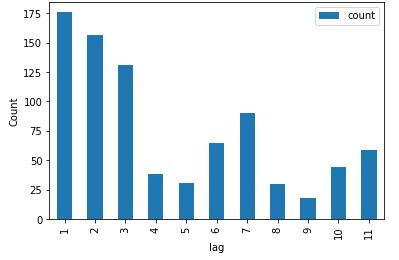
\includegraphics[width=0.8\linewidth]{Figure/Data_PartialAutocorrelation.JPG}
	\caption{Lag level per group} 
	\label{fig:LagLevel}
\end{figure}

\subsubsection{Generaci\'on del dataset de entrenamiento}
%%---------------------- Reempleazar
Lorem ipsum dolor sit amet, consectetur adipiscing elit, sed do eiusmod tempor incididunt ut labore et dolore magna aliqua. Ut enim ad minim veniam, quis nostrud exercitation ullamco laboris nisi ut aliquip ex ea commodo consequat. Duis aute irure dolor in reprehenderit in voluptate velit esse cillum dolore eu fugiat nulla pariatur. Excepteur sint occaecat cupidatat non proident, sunt in culpa qui officia deserunt mollit anim id est laborum.
%%---------------------
\begin{figure}[h!]
	\centering
	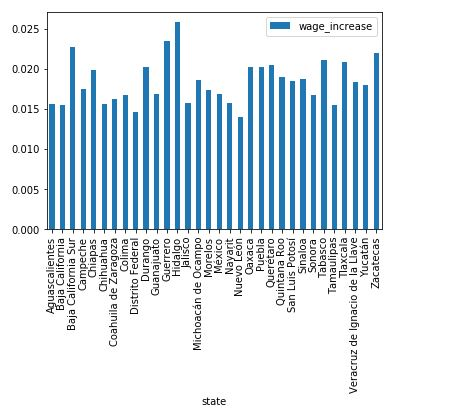
\includegraphics[width=0.8\linewidth]{Figure/Data_TrainingDataset.JPG}
	\caption{Lag level per group} 
	\label{fig:InitialData}
\end{figure}

%%---------------------- Reempleazar
Lorem ipsum dolor sit amet, consectetur adipiscing elit, sed do eiusmod tempor incididunt ut labore et dolore magna aliqua. Ut enim ad minim veniam, quis nostrud exercitation ullamco laboris nisi ut aliquip ex ea commodo consequat. Duis aute irure dolor in reprehenderit in voluptate velit esse cillum dolore eu fugiat nulla pariatur. Excepteur sint occaecat cupidatat non proident, sunt in culpa qui officia deserunt mollit anim id est laborum.
%%---------------------
\begin{figure}[h!]
	\centering
	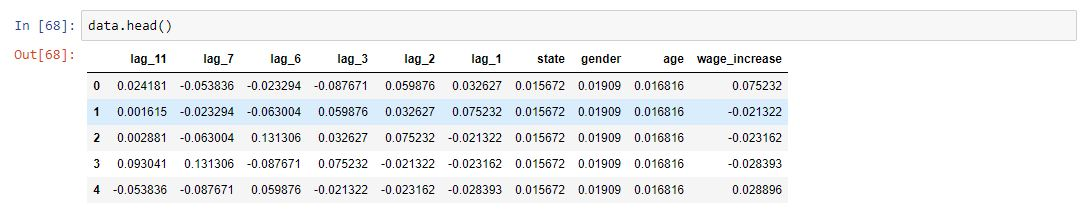
\includegraphics[width=1\linewidth]{Figure/DataSet_TrainingDataset.JPG}
	\caption{Lag level per group} 
	\label{fig:TrainingDataSet}
\end{figure}


\subsection{Descripci\'on del Modelo a Utilizar}

\subsubsection{Regresi\'on Lineal}

\subsubsection{Decision Tree}
Los modelos de \'arbol de Regresi\'on y Clasificaci\'on (C&RT, Classification & Regression Trees), fueron introducidos en la Estad\'istica por Breiman et al. (1984). Diversos autores utilizan el t\'ermino ``modelos de \'arbol de regresi\'on'' cuando la variable respuesta es cuantitativa y el de ``modelos de \'arbol de clasificaci\'o'' cuando \'esta es cualitativa. 
Decision tree Regression es un algoritmo de aprendizaje dentro del grupo de aprendizaje supervisado. Este se caracteriza por particionar o dividir los datos en varias clasificaciones de grupos homog\'eneos respecto a la variable, creando iteraciones de estas clasificaciones del DataFrame hasta conseguir el mejor resultado posible. Este m\'etodo utiliza los datos de entrenamiento de periodos anteriores y los entrena para conseguir clasificar los nuevos datos.
Dentro de las ventajas de este algoritmo se encuentran las siguientes:
Facilidad al comprender y explorar datos, debido a su clasificaci\'on y traficaci\'on. 
Dentro de las ventajas de este algoritmo se encuentran:
Los sobreajustes son muy comunes en estos modelos y al usar variables continuas, se tiene por sobre entendido que se perder\'a precisi\'on.

\subsubsection{Random Forest Regressor}


\subsubsection{XGBoost}
Es muy parecido al modelo Random Forest, pero esta vez los \'arboles tienen asociadas una funci\'on de p\'erdidas que tienen que minimizar (o maximizar) para conseguir los mejores resultados (por ello la palabra Boosting).
Est\'a basado o es muy parecido al \'arbol de decisi\'on y es una evoluci\'on entre la clasificaci\'on y la regresi\'on  este se basa en impulsar  para maximizar o minimizar la funci\'on de p\'erdidas trabaja sobre bases de datos de gran tamaño as\'i como m\'ultiples variables algo importante es que admite missing values  por lo mencionado anteriormente se debe tener en cuenta el equipo para  correr bases de datos extensas y usar muchas variables, es recomendable saber las variables que m\'as aportan al algoritmo.

Este clasifica o pron\'ostica sobre la variable objetivo, utiliza un set de datos utilizando los los \'arboles de decisiones para potencializar los resultados en base a un procesamiento secuencial y con una funci\'on de p\'erdida  que minimiza el error en consecuencia es un pronosticador fuerte. Como en todo algoritmo se deben ajustar los par\'ametros para obtener un m\'inimo error de precisi\'on


\subsection{Delimitaciones}
\subsubsection{Datos}
La serie estad\'istica presenta la poblaci\'on que tiene una actividad economica subordinada y remunerada del pais para cada una de las entidades federativas, desglosada por sexo, grupos de edad y cual es el nivel de ingreso de la poblaci\'on.\ref{fig:TrainingDataSet}\cite{datosAbiertos_2019}
\subsubsection{Temporales}
El presente es un estudio longitudinal en donde los datos de 2005 a 2018 se utilizar\'an como entrada para poder predecir el de salario, del 2019

%\subsubsection{Te\'oricas}